\chapter{GCC}
\section{GCC编译过程与实质}
\par GCC的编译包含了几个步骤:
\begin{enumerate}
  \item 预处理
  \item 编译
  \item 汇编
  \item 链接
\end{enumerate}

其中预处理,最主要的工作就是将所有的源代码准备,并且将源代码当中的宏定义进行替换。
而编译,则是使用cc1命令,对c文件进行编译,即将c文件处理成s(汇编文件)
\begin{code-block}{c}
# 实际上使用的是 cc1命令
 /usr/libexec/gcc/x86_64-redhat-linux/4.8.5/cc1 -quiet -v test.c \
    -quiet -dumpbase test.c -mtune=generic -march=x86-64 -auxbase test \
    -version -o /tmp/ccHGK1zq.s

# 上述的命令实际上是由gcc的命令完成或者直接调用
gcc -S -o test.s test.c
\end{code-block}

而汇编则是将汇编文件进行编译,翻译成字节码文件
\begin{code-block}{c}
# 实际上使用的是as命令
as -v --64 -o /tmp/ccWcmHvw.o /tmp/ccHGK1zq.s
# 上述的命令实际上是由gcc的命令完成或者直接调用
gcc -c -o test.o test.c
\end{code-block}

最后一步,则是将汇编生成的字节码文件,转换成可执行的二进制文件
\begin{code-block}{c}
# 实际上使用的是as命令
/usr/libexec/gcc/x86_64-redhat-linux/4.8.5/collect2 --build-id --no-add-needed ...
# 上述的命令实际上是由gcc的命令完成或者直接调用
gcc -o test.out test.o
\end{code-block}

GCC的编译参数,可以分为静态编译(-static)与动态编译(-shared)。静态编译会将所有的
依赖库合并为一个可执行文件,占用空间比较大;而动态编译则是生成动态的问题,生成的文件较小。
默认情况下,gcc使用动态编译的方式。
\begin{code-block}{c}
# 强制使用静态编译的方式需要使用参数-static,另外,依赖于glibc-static这个类库
gcc -static -o test.out test.o
\end{code-block}

动态编译(-shared)则通常与-fPIC(相对位置无关)参数一同使用。

\section{制作静态链接库}
静态链接库的生成过程以及使用方式大致如下:
\begin{enumerate}
  \item 生成目标文件(.o)
  \item 将静态库(.a)与目标文件打包(ar)
  \item 调用静态链接库:gcc -o target source.c -L
\end{enumerate}

具体操作可见如下

\begin{code-block}{c}
// testlib.c
#include <stdio.h>
unsigned int add(unsigned int a, unsigned int b)
{
        return a + b;
}

// testmain.c
#include <stdio.h>
unsigned int add(unsigned int, unsigned int);
int main(int argc, char * argv[])
{
        unsigned int a = 10;
        unsigned int b = 20;
        printf("%u\n", add(a, b));
        return 0;
}
\end{code-block}

然后将上述代码testlib.c转换成目标文件
\begin{code-block}{bash}
gcc -o testlib.o testlib.c
\end{code-block}

随之将其进行归档打包,生成静态链接库文件
\begin{code-block}{bash}
ar crv testlib.a testlib.o
\end{code-block}

使用静态链接库文件进行代码编译
\begin{code-block}{bash}
gcc -o testmain testmain.c -L./ testlib.a
\end{code-block}

\section{制作动态链接库}
动态链接库的生成过程以及使用方式大致如下:
\begin{enumerate}
  \item 生成位置无关的目标代码(-fPIC)
  \item 生成动态链接库文件 gcc -shared -o *.so *.o
  \item 调用动态链接库 gcc -o target source.c -L[path] *.so
\end{enumerate}

具体操作可见如下

\begin{code-block}{c}
// testlib.c
#include <stdio.h>
unsigned int add(unsigned int a, unsigned int b)
{
        return a + b;
}

// testmain.c
#include <stdio.h>
unsigned int add(unsigned int, unsigned int);
int main(int argc, char * argv[])
{
        unsigned int a = 10;
        unsigned int b = 20;
        printf("%u\n", add(a, b));
        return 0;
}
\end{code-block}

首先是生成位置无关的目标代码
\begin{code-block}{bash}
gcc -fPIC -c -o testlib.o testlib.c
\end{code-block}

随后生成动态链接库文件
\begin{code-block}{bash}
gcc -shared -o testlib.so testlib.o
\end{code-block}

然后编译main文件
\begin{code-block}{bash}
gcc -o testmain testmain.c -L./ testlib.so
\end{code-block}

最后执行文件
\begin{code-block}{bash}
# 由于Linux下,默认的so文件全部放在$LD_LIBRARY_PATH,即/usr/lib和/usr/lib64下,
# 因此,链接到自己的so文件时,要么将这个so放到规定的路径下,要么使用环境变量的模式进行加载
LD_LIBRARY_PATH=.:$LD_LIBRARY_PATH ./testmain

# 使用规定目录的方式(x86_64)
# mv testlib.so /lib64
# ldconfig
# ./testmain

# 使用配置文件的方式
# echo `pwd` >> /etc/ld.so.conf
# ldconfig
# ./testmain
\end{code-block}

\section{编译GCC}
GCC的编译需要依赖以下几个软件包:
\begin{itemize}
  \item GMP:ftp://gcc.gnu.org/pub/gcc/infrastructure/gmp-6.1.0.tar.bz2
  \item MPFR:ftp://gcc.gnu.org/pub/gcc/infrastructure/mpfr-3.1.4.tar.bz2
  \item MPC:ftp://gcc.gnu.org/pub/gcc/infrastructure/mpc-1.0.3.tar.gz
  \item m4
\end{itemize}

\section{定义函数别名}
在GCC当中提供了一系列的扩展功能,包含了定义方法的别名。函数的别名可以是强引用,也可以是弱引用。
\begin{code-block}{c}
void __swap_object(void * first, void * last, size_t size)
{
    void * tmp = malloc(size);
    memcpy(tmp, first, size);
    memcpy(first, last, size);
    memcpy(last, tmp, size);
    free(tmp);
}

// 弱引用别名
void swap_weak(void * first, void *last, size_t size)
        __attribute__ ((weak, alias("__swap_object")));
// 强引用别名
void swap_strone(void * first, void *last, size_t size)
        __attribute__ ((alias("__swap_object")));
\end{code-block}

\section{标记函数被废弃}
在GCC也支持标记函数为废弃,来警示相关人员不要使用这样的函数。
\begin{code-block}{c}
void print_hello() __attribute__ ((deprecated));
void print_hello()
{
    printf("hello\n");
}
\end{code-block}

通过以上的方式进行标记时候,在调用printf\_hello这个方法的时候,编译过程中会提示
如下的信息:
\begin{code-block}{bash}
test.c:74:5: 警告:‘print_hello’ is deprecated [-Wdeprecated-declarations]
     print_hello();
     ^~~~~~~~~~~
test.c:46:6: 附注:在此声明
 void print_hello()
\end{code-block}

\section{特殊的GCC扩展}
有的时候,我们可能需要在执行main方法之前执行一些动作,在执行完main方法之后,再
进行一些扫尾的动作。GCC提供了这样的支持。
\begin{code-block}{c}
// 进入main方法之前就执行该方法
void hello() __attribute__ ((constructor));
void hello()
{
    printf("hello\n");
}

// 退出main方法之后,执行该方法
void bye() __attribute__ ((destructor));
void bye()
{
    printf("bye\n");
}
int main(int argc, char * argv[])
{
    return 0;
}
\end{code-block}

以上代码编译执行之后,其输出为:
\begin{code-block}{bash}
helllo
bye
\end{code-block}

\section{GCC内置函数}
GCC提供了一系列的内置函数,用于进行优化程序。

\begin{outline}[enumerate]

\1 \_\_builtin\_types\_compatible\_p

该函数为GCC的扩展函数,用于判断2个数据的类型是否相同。其原型定义如下:
\begin{code-block}{c}
  int __builtin_types_compatible_p(type_a, type_b);
\end{code-block}

在真正的使用当中,可以用于进行宏定义,来判断传递的参数是否为需要的类型:
\begin{code-block}{c}
// 判断传递的参数是否为数组
#define BUILD_BUG_ON_ZERO(e) (sizeof(char[1 - 2 * !!(e)]) - 1)
#define __same_type(a, b) __builtin_types_compatible_p(typeof(a), typeof(b))
#define __must_be_array(a) BUILD_BUG_ON_ZERO(__same_type((a), &(a)[0]))
\end{code-block}

关于BUILD\_BUG\_ON\_ZERO在前面的已经仔细讲解过,其主要作用就是用来发现编译时的错误,
\_\_same\_type宏定义用于判断传入的参数是否是相同的数据类型,a表示原始的数据,(a)[0]表示
取a数组的第0个元素,\&(a)[0]表示对a数组的第0个元素取地址,因此,\_\_same\_type((a), \&(a)[0])
的作用就是,通过\&(a)[0]这个操作,来区分数组和其他类型,如果数据a可以执行该操作,可以认为
a是一个数组或指针,反之,就会报错,从而在编译时刻就发现错误。同样的,该宏定义还可以区分数组与指向数组
的指针:typeof(a)返回的是数组类型,而typeof(\&a[0])返回的则是指针类型。

\begin{code-block}{c}
int a[] = {1,2,3};
__must_be_array(a);
float b[] = {1,2,3};
__must_be_array(b);
int c = 123;
int *d = &c;
__must_be_array(d); // 编译时提示错误
int *e = a;
__must_be_array(e); // 同样是编译提示错误
\end{code-block}

\1 \_\_arm\_\_

该属性用于判断当前的编译器或者代码是否针对arm结构,具体的使用如下:
\begin{code-block}{c}
#if defined(__arm__)
        printf("This is build for arm arch\n");
#endif
\end{code-block}
除了针对ARM之外,还有其他的一些特殊的宏定义,大致如下:
\begin{enumerate}
  \item 针对x86-64:\_\_amd64\_\_, \_\_amd64, \_\_x86\_64\_\_, \_\_x86\_64
  \item 针对x86:\_\_i386,\_\_i386\_\_
  \item 针对arm:
  \begin{itemize}
  \item \_\_arm\_\_
  \item \_\_ARM\_ARCH\_2\_\_
  \item \_\_ARM\_ARCH\_3\_\_
  \item \_\_ARM\_ARCH\_3M\_\_
  \item \_\_ARM\_ARCH\_4T\_\_
  \item \_\_TARGET\_ARM\_4T
  \end{itemize}
  \item 针对arm64:\_\_aarch64\_\_
  \item 针对alpha:\_\_alpha\_\_
\end{enumerate}
这些宏定义可以在内核代码以及普通代码当中直接使用。

\end{outline}

\section{Makefile}
Makefile当中包含了一些特殊的系统变量,这些特定的系统变量如表\colorunderlineref{tab:macro_of_makefile}所示
\begin{table}[H]
  \caption{GCC的特定系统变量}
  \label{tab:macro_of_makefile}
  \rowcolors{2}{green!80!yellow!50}{green!70!yellow!40}
  \begin{tabularx}{\textwidth}{|X|X|}
  \hline
  \centering 表达式& \centering\arraybackslash 说明\\ \hline
  \centering \$* & 不包含扩展名的目标文件名称 \\
  \centering \$< & 第一个依赖文件名称\\
  \centering \$? & 所有时间戳比目标文件晚的依赖文件\\
  \centering \$@ & 目标文件完整名称\\
  \centering \$\^{} & 所有不重复的依赖文件\\ \hline
  \end{tabularx}
\end{table}

比如有如下的一段代码
\begin{code-block}{make}
TARGET = testmain
OBJS = testmain.o testlib.o
testmain : $(OBJS)
        $(CC) -o $@ $^
\end{code-block}

在上述代码当中\$\@就表示testmain这个目标,\$\^则表示testmain的依赖文件,即\$(OBJS)所代表的testmain.o和testlib.o文件

默认的,Makefile当中执行的每一行代码都会在屏幕当中显示出来。如果不需要显示,则只需要在命令前添加@符号即可,如下:
\begin{code-block}{make}
TARGET = testmain
OBJS = testmain.o testlib.o
testmain : $(OBJS)
        @$(CC) -o $@ $^
\end{code-block}

Makefile本身也支持嵌套。假设现在有一个工程,其目录结构如图\colorunderlineref{fig:submake}所示。
\begin{figure}[H]
  \centering
  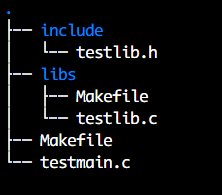
\includegraphics[scale=1.0]{make.png}
  \caption{Makefile嵌套}
  \label{fig:submake}
\end{figure}

则在编译时,我们可以使用Makefile进行统一的嵌套管理
\begin{code-block}{make}
# 外层的Makefile
TARGET = testmain
OBJS = testmain.o libs/testlib.o
INC = include
testmain : $(OBJS)
        @$(CC) -o $@ $^
testmain.o: testmain.c
        $(CC) -I$(INC) -c $^
libs/testlib.o:
        $(MAKE) -C libs #嵌套执行libs下的makefile
.PHONY: clean
clean:
        rm -rf $(OBJS) $(TARGET)

#libs当中的Makefile
OBJS = testlib.o
INC = ../include
testlib.o: testlib.c
        $(CC) -I$(INC) -c $^
.PHONY: clean
clean:
        rm -rf $(OBJS)
\end{code-block}

当然,也可以单独执行每个路径下的Makefile
